\documentclass{article}
\usepackage{graphicx}

\usepackage{algorithm}
\usepackage{algpseudocode}





\title{nbWave:  3D Surface Waves in a Narrow Band Volume}
\author{Jerry Tessendorf}

\def\xvec{\textbf{x}}
\def\fvec{\textbf{f}}
\def\gvec{\textbf{g}}
\def\uvec{\textbf{u}}
\def\Xvec{\textbf{X}}
\def\yvec{\textbf{y}}
\def\kvec{\textbf{k}}
\def\nhat{\hat{\textbf{n}}}
\def\mmm{{\cal M}}
\def\what{{\hat{\omega}}}
\def\dt{\Delta t}
\def\dx{\Delta x}
\def\dy{\Delta y}
\def\inabla{\nabla^{*}}
\def\tnabla{\nabla_t}

\def\dx{\Delta x}
\def\dy{\Delta y}
\def\dz{\Delta z}
\def\xhat{\hat{\textbf{x}}}
\def\yhat{\hat{\textbf{y}}}
\def\zhat{\hat{\textbf{z}}}


\begin{document}
\maketitle

\begin{abstract}
This evolving note describes an approach to generalizing the eWave algorithm to solving for waves on an arbitrary surface  from the Bernoulli equations using a small band of volume around the surface.
\end{abstract}
%\tableofcontents
%\newpage

\section{nbWave Dynamics}

The dynamical equations for iWave are essentially Bernoulli's equations for displacements of a flat surface.  The fundamental dynamical fields are the velocity potential $\phi$ and the displacement height $h$, which satisfy the equations\footnote{The original paper on iWave used a single second order differential equation for the height, whereas this system is two first order differential equations for height and velocity potential.  Mathematically the two forms are identical, but numerical solution strategies differ for the two forms.  iWave was also implemented in this coupled-first order form but unpublished. The coupled first-order form is more stable and amenable to a broader set of solver strategies.}
\begin{eqnarray}
\frac{\partial \phi(\xvec,t)}{\partial t} &=& -g h(\xvec,t) \\
\frac{\partial h(\xvec,t)}{\partial t} &=& \frac{\partial \phi(\xvec,t)}{\partial y}  \\
\nabla^2 \phi(\xvec,t) &=& 0
\end{eqnarray}
The last equation is used in the iWave algorithm to define the vertical gradient of $\phi$ as
\begin{equation}
\frac{\partial \phi}{\partial y}\ \equiv\ \sqrt{-\left(\frac{\partial^2}{\partial x^2} \ +\ \frac{\partial^2}{\partial z^2}\right)} \ \phi \label{fractiongrad}
\end{equation}

Generalizing this dynamics to take place on an arbitrary surface requires several generalizations: 
\begin{enumerate}
\item The arbitrary surface needs to be defined in a robust way.  We choose to use an implicit surface $S_B(\xvec,t)$ for the base surface that is input to this problem, and $S_E(\xvec,t)$ for extension of the surface induced by the surface waves.  The complete surface is $S_B(\xvec,t) + S_E(\xvec,t)$.

\item The displacement in the iWave algorithm is no longer a simple normal displacement.  We need to generalize it to a vector field $\Xvec_E(\xvec,t)$.  
\end{enumerate}

In this generalization, we also want to include the fact that the base surface is evolving by advection from a velocity field $\uvec_B(\xvec,t)$.  We also want to include more complex forcing, including the nonlinear Bernoulli term that iWave ignores, surface tension, and gravity.

These considerations lead to the following set of equations for the generalization of iWave
\begin{eqnarray}
\frac{\partial \phi(\xvec,t)}{\partial t} \ +\ \uvec_B(\xvec,t)\cdot\nabla\phi(\xvec,t) &=& -\gvec\cdot\Xvec_E(\xvec,t)
\ +\  f_{ST}  \label{phieqn}\\
\frac{\partial \Xvec_E(\xvec,t)}{\partial t} \ +\ \uvec_B(\xvec,t)\cdot\nabla\Xvec_E(\xvec,t) &=& -\inabla\phi(\xvec,t) \label{xeeqn}  \\
\nabla^2\phi(\xvec,t) &=& 0 \\
\frac{\partial S_E(\xvec,t)}{\partial t} \ +\ \uvec_B(\xvec,t)\cdot\nabla S_E(\xvec,t) &=& -\nabla S_B(\xvec,t)\cdot\inabla\phi(\xvec,t) \label{seqn}
\end{eqnarray}
The surface tension force $f_{ST}$ is
\begin{equation}
f_{ST} \ =\  \sigma\  \nabla\cdot\left(  \frac{\nabla S_B + \nabla S_E}{ |  \nabla S_B + \nabla S_E |  } - \alpha  \frac{\nabla S_B}{ |  \nabla S_B |  } \right) \ \textbf{1}(S_B+S_E)
\end{equation} 
The quantity $\textbf{1}(S)$ is zero away from the surface, one at the surface, and ramps smoothly between through a desired thickness $\epsilon$, usually taken to be proportional to grid spacing.  This function comes from spatial integrating through the surface the Dirac delta function enforcing surface tension only on the surface.  A common, but not unique, choice is
\begin{equation}
\textbf{1}(S)\ \equiv\ \left\{  \begin{array}{ll}
                                      0 & |S| > \epsilon  \\
                                      \frac{1}{2}\left( 1\ +\ \cos\left(\frac{\pi S}{2\epsilon}\right)  \right) & |S| \leq \epsilon
                                \end{array}  \right.
\end{equation}
The parameter $\sigma$ is the physical coefficient for the strength of surface tension.  The parameters $0\leq\alpha,\beta\leq 1$ are unphysical control parameters for adjusting the surface tension and nonlinear Bernoulli forcing.
See section \ref{derivation} for a derivation of these equations from the Navier-Stokes equations. The object $\inabla$ is an {\em incompressible gradient} defined in section \ref{igradient}.




\section{Incompressible Gradient}\label{igradient}

In the eWave algorithm, Laplace's equation is not directly tackled in the numerics.  Instead, it is used to define the vertical derivative as a fractional derivative in equation \ref{fractiongrad}.  Once this form is employed, explicit enforcement of Laplace's equation is not necessary.  This reduces the complexity of some aspects of the dynamics problem, but does not eliminate the difficulties associated with incompressibility, because the vertical derivative is given the unusual fractional derivative form that must be evaluated via FFTs or convolution.  

In the nbWave scenario, Laplace's equation is again present, but we want to remove it from the collection of equations to solve numerically. But this scenario does not have the horizontally uniform conditions that eWave benefits from.  The arbitrary surface $S_B$ breaks up this uniformity and makes it less attractive to try the fractional derivative approach.  

In this section three approaches to this issue are presented.  The result of all of them is the construction of gradient operator that is explicitly constrained to support Laplace's equation.  This gradient operator is labelled an {\em incompressible gradient} and given the symbol $\inabla$.

\subsection{Fractional Derivative}
One approach is to apply the eWave approach in this situation. The component of the gradient perpendicular to the surface is defined as $\partial_n \equiv \nhat_B\cdot\nabla$, where $\nhat_B$ is the unit surface normal. The transverse portion of the gradient is
\begin{equation}
\tnabla\  \equiv\ \nabla\ -\ \nhat_B\partial_n 
\end{equation}
This expression gives rise to a laplacian of the form
\begin{eqnarray}
\nabla^2 &=& \left( \nhat_b\partial_n \ +\ \tnabla  \right)\cdot \left( \nhat_b\partial_n \ +\ \tnabla  \right) \nonumber \\
&=& \partial_n^2 \ +\ \tnabla^2 \ + \kappa_B \partial_n
\end{eqnarray} 
where $\kappa_B$ is the curvature of the surface: $\kappa_B \equiv \nabla\cdot\nhat_B$.  Treating this as a quadratic equation for $\partial_n$, the perpendicular gradient that satisfies Laplace's equation is
\begin{equation}
\partial_n \ =\ -\frac{\kappa_B}{2}\ +\ \sqrt{ \left(\frac{\kappa_B}{2}\right)^2  - \tnabla^2     }
\end{equation}
The incompressible gradient follows as
\begin{equation}
\inabla\phi \ =\ \tnabla\phi \ + \ \nhat_B \left( -\frac{\kappa_B}{2}\ +\ \sqrt{ \left(\frac{\kappa_B}{2}\right)^2  - \tnabla^2 } \right)\phi
\end{equation}

There are several things to note about this: 
\begin{enumerate}
\item In the limit of a flat surface, $\kappa_B=0$ and this expression reduces to the eWave fractional derivative in equation \ref{fractiongrad}.

\item The curvature and the transverse gradient are location-specific, and so any implementation will not be able to exploit spatial homogeneity in any way.

\item Like the situation in iWave, implementing such an operator requires a convolution kernel, and without spatial homogeneity, the kernel must be constructed at each point of the surface.

\end{enumerate} 
The last two issues make this approach difficult to use.

\subsection{Finite Difference}
An alternative, more attractive, approach works directly with the grid structure of the data.  Assume a rectangular grid structure with grid point spacing $\dx, \dy, \dz$.  The issue of imposing a narrow band active region is addressed in section \ref{nbsection}.  The gradient of $\phi$ using a central difference is
\begin{eqnarray}
\nabla\phi(\xvec) &=& \left(  \frac{\phi(\xvec + \dx \xhat) - \phi(\xvec - \dx \xhat) }{2\dx},\right. \nonumber \\
&&   \frac{\phi(\xvec + \dy \yhat) - \phi(\xvec - \dy \yhat) }{2\dy}, \nonumber \\
&& \left.  \frac{\phi(\xvec + \dz \zhat) - \phi(\xvec - \dz \zhat) }{2\dz}  \right)
\end{eqnarray}
At the same time, Laplace's equation on a rectangular grid is commonly written as
\begin{eqnarray}
0 \ =\ \nabla^2\phi(\xvec) &=& \frac{\phi(\xvec + \dx \xhat) -2\phi(\xvec) + \phi(\xvec - \dx \xhat) }{\dx^2} \nonumber \\
&+&                     \frac{\phi(\xvec + \dy \yhat) -2\phi(\xvec) + \phi(\xvec - \dy \yhat) }{\dy^2} \nonumber \\
&+&                     \frac{\phi(\xvec + \dz \zhat) -2\phi(\xvec) + \phi(\xvec - \dz \zhat) }{\dz^2}
\label{gridlaplace}
\end{eqnarray}

The incompressible gradient on a grid comes from using Laplace's equation to fix terms in the gradient. For example, the forward evaluations $\phi(\xvec+\dx\xhat)$, etc. can be expressed as
\begin{eqnarray}
 \phi(\xvec + \dx \xhat) &=& 2\phi(\xvec) - \phi(\xvec - \dx \xhat) \nonumber \\
&-& \frac{\dx^2}{\dy^2}\left( \phi(\xvec + \dy \yhat) -2\phi(\xvec) + \phi(\xvec - \dy \yhat) \right) \nonumber \\
&-& \frac{\dx^2}{\dz^2}\left(   \phi(\xvec + \dz \zhat) -2\phi(\xvec) + \phi(\xvec - \dz \zhat) \right)
\end{eqnarray}
\begin{eqnarray}
\phi(\xvec + \dy \yhat) &=& 2\phi(\xvec) - \phi(\xvec - \dy \yhat) \nonumber \\
&-& \frac{\dy^2}{\dx^2}\left( \phi(\xvec + \dx \xhat) -2\phi(\xvec) + \phi(\xvec - \dx \xhat) \right) \nonumber \\
&-& \frac{\dy^2}{\dz^2}\left(   \phi(\xvec + \dz \zhat) -2\phi(\xvec) + \phi(\xvec - \dz \zhat) \right)
\end{eqnarray}
\begin{eqnarray}
\phi(\xvec + \dz \zhat) &=& 2\phi(\xvec) - \phi(\xvec - \dz \zhat) \nonumber \\
&-& \frac{\dz^2}{\dy^2}\left( \phi(\xvec + \dy \yhat) -2\phi(\xvec) + \phi(\xvec - \dy \yhat) \right) \nonumber \\
&-& \frac{\dz^2}{\dx^2}\left(   \phi(\xvec + \dx \xhat) -2\phi(\xvec) + \phi(\xvec - \dx \xhat) \right)
\end{eqnarray}
Inserting these into the gradient, the incompressible gradient is
\begin{eqnarray}
\inabla\phi(\xvec) &=& \left(  \frac{\phi(\xvec) - \phi(\xvec - \dx \xhat) }{\dx},
  \frac{\phi(\xvec) - \phi(\xvec - \dy \yhat) }{\dy}, 
  \frac{\phi(\xvec) - \phi(\xvec - \dz \zhat) }{\dz}  \right)  
\label{gridigrad} \\
&-& \frac{\dx}{2}\ \xhat\ \left( \frac{ \phi(\xvec + \dy \yhat) -2\phi(\xvec) + \phi(\xvec - \dy \yhat)}{\dy^2} +  \frac{ \phi(\xvec + \dz \zhat) -2\phi(\xvec) + \phi(\xvec - \dz \zhat)}{\dz^2} \right) \nonumber \\
&-& \frac{\dy}{2}\ \yhat\ \left( \frac{ \phi(\xvec + \dx \xhat) -2\phi(\xvec) + \phi(\xvec - \dx \xhat)}{\dx^2} +  \frac{ \phi(\xvec + \dz \zhat) -2\phi(\xvec) + \phi(\xvec - \dz \zhat)}{\dz^2} \right) \nonumber \\
&-& \frac{\dz}{2}\ \zhat\ \left( \frac{ \phi(\xvec + \dy \yhat) -2\phi(\xvec) + \phi(\xvec - \dy \yhat)}{\dy^2} +  \frac{ \phi(\xvec + \dx \xhat) -2\phi(\xvec) + \phi(\xvec - \dx \xhat)}{\dx^2} \right) \nonumber 
\end{eqnarray}
Even though the gradient is based on central differences, and the Laplacian is built symmetrically, the first term of this expression is the forward difference expression for a gradient.  The remaining terms are second-order derivative corrections that enforce incompressibility.

The incompressible gradient form in equation \ref{gridigrad} is simple to implement in a system based on rectangular gridded data, even when the grid supports narrow band logic.  Also the choice of substituting for the forward evaluation was arbitrary.  The backward evaluation could have been the target of substitution, and the choice could be made component by component.  This flexibility can be exploited to simplify boundary condition issues substantially (section \ref{boundaryconditions}).  

One of the potential issues with equation \ref{gridigrad} is that the gradient and laplacian expressions may not be sufficiently accurate to give good solutions to incompressiblity.  These finite difference expressions can be extended to higher order as desired to give higher quality results.  

Illustrating with a 1-D function $f(x)$, the Taylor expansion
\begin{equation}
f(x+y) \ =\ \sum_{k=0}^{\infty}\frac{y^k}{k!}f^{(k)}(x)
\end{equation}
can be used to assemble any order finite-difference approximation.  Here $f^{(k)}$ is the $k-th$ derivative of the function.  A derivative can be represented as a finite sum of $2N$ terms:
\begin{equation}
\frac{d}{dx}f(x)\ \approx\ \sum_{n=-N}^{N}\ a_n\ f(x+n\dx)
\end{equation}
with suitably chosen coefficients $a_n$.  The approach to fixing their values comes from applying
the Taylor expansion to this approximation to get
\begin{equation}
\sum_{k=0}^{\infty} \ \frac{\dx^k}{k!} f^{(k)}(x) \ \sum_{n=-N}^{N} n^k\ a_n
\end{equation}
If this is intended to represent the first derivative, the coefficients must be fixed by the series of equations
\begin{eqnarray}
\sum_{n=-N}^{N} \ a_n &=& 0 \label{basea}\\
\sum_{n=-N}^{N} n\ a_n &=& \frac{1}{\dx} \label{onea}\\
\sum_{n=-N}^{N} n^k\ a_n &=& 0\ \ \ \  k>1 \label{othera}
\end{eqnarray}
Equation \ref{basea} and all equations \ref{othera} for even $k$ are satisfied if the coefficients are antisymmetric, i.e. $a_{-n} = -a_n$. This fixed $a_0=0$. Further, it makes sense to scale the coefficients by $a_n = \alpha_n/\dx$.  Once these choices are made, the remaining equations are
\begin{eqnarray}
\sum_{n=1}^{N} n\ \alpha_n &=& \frac{1}{2} \label{oneaa}\\
\sum_{n=1}^{N} n^{2k+1}\ \alpha_n &=& 0\ \ \ \  k>1 \label{otheraa}
\end{eqnarray}
The coefficients for choices of $N$ up to 4 are shown in table \ref{derivativecoefficients}, and for $N=5$ through $N=8$ in table \ref{derivativecoefficients5-8}.
\begin{table}
\begin{center}
\footnotesize
\begin{tabular}{|c|c|c|c|c|}\hline
           & $N=1$ & $N=2$ & $N=3$ & $N=4$ \\ \hline
$\alpha_1$ & 0.5 &   6.666666666666666296592e-01 & 0.75                 &  0.8  \\ \hline
$\alpha_2$ &     &  -8.333333333333332870740e-02 & -0.15                & -0.2 \\ \hline
$\alpha_3$ &    &                         & 1.666666666666666296592e-02 & 3.809523809523807785782e-02  \\ \hline
$\alpha_4$ &    &                         &                             & -3.571428571428579123309e-03 \\ \hline
\end{tabular}
\end{center}
\caption{Coefficients for finite difference derivatives up to $N=4$.}\label{derivativecoefficients}
\end{table}
\begin{table}
\begin{center}
\footnotesize
\tiny
\begin{tabular}{|c|c|c|c|c|}\hline 
           & $N=5$ & $N=6$ & $N=7$ & $N=8$ \\ \hline
$\alpha_1$ &  8.333333333333301506940e-01  &  8.571428571428428844214e-01  & 8.749999999997666311202e-01    & 8.888888888890622563821e-01   \\ \hline
$\alpha_2$ & -2.380952380952371660872e-01  &  -2.678571428571295820475e-01 & -2.916666666664030627132e-01   & -3.111111111113007976492e-01 \\ \hline
$\alpha_3$ & 5.952380952380949968861e-02   & 7.936507936506739802063e-02   & 9.722222222201161445643e-02    & 1.131313131315020842349e-01  \\ \hline
$\alpha_4$ & -9.920634920635062331540e-03  &  -1.785714285714170776465e-02 &  -2.651515151521397634093e-02  & -3.535353535356308696258e-02 \\ \hline
$\alpha_5$ & 7.936507936507907227594e-04   & 2.597402597401952516892e-03   &  5.303030303006155132817e-03   & 8.702408702345020702351e-03   \\ \hline
$\alpha_6$ &                               & -1.803751803751641390964e-04  &  -6.798756798778969601127e-04  & -1.554001554001562023302e-03   \\ \hline
$\alpha_7$ &                               &                               &  4.162504162505081361893e-05   & 1.776001776006136932424e-04   \\ \hline
$\alpha_8$ &                               &                               &                                & -9.712509712526897105722e-06  \\ \hline
\end{tabular}
\end{center}
\caption{Coefficients for finite difference derivatives in the range $N=5-8$.}\label{derivativecoefficients5-8}
\end{table}

The same logic and steps apply to approximating the second derivative.  The finite difference expression has coefficients $b_n$
\begin{equation}
\frac{d^2}{dx^2}f(x)\ \approx\ \sum_{n=-N}^{N}\ b_n\ f(x+n\dx)
\end{equation}
and the Talor expansion of this as
\begin{equation}
\sum_{k=0}^{\infty} \ \frac{\dx^k}{k!} f^{(k)}(x) \ \sum_{n=-N}^{N} n^k\ b_n
\end{equation}
leads to the set of equations
\begin{eqnarray}
\sum_{n=-N}^{N} \ b_n &=& 0 \\
\sum_{n=-N}^{N} n\ b_n &=& 0 \\
\sum_{n=-N}^{N} n^2\ b_n &=& \frac{2}{\dx^2} \\
\sum_{n=-N}^{N} n^k\ b_n &=& 0\ \ \ \ \ k>2 \\
\end{eqnarray}
In this situation large numbers of equations are eliminated by making the coefficients symmetric, i.e. $b_{-n}=b_n$.  The scaling is $b_n=\beta_n/\dx^2$.  The reduced equations are:
\begin{eqnarray}
2\sum_{n=1}^{N} \ \beta_n &=& -\beta_0\\
\sum_{n=1}^{N} n^2\ \beta_n &=& 1 \\
\sum_{n=1}^{N} n^{2k}\ \beta_n &=& 0\ \ \ \ \ k>1 \\
\end{eqnarray}
These coefficients for choices of $N$ up to 3 are shown in table \ref{secondcoefficients}.
\begin{table}
\begin{center}
\begin{tabular}{|c|c|c|c|}\hline
          & $N=1$ & $N=2$   & $N=3$ \\ \hline
$\beta_0$ & $-2$&  $-15/6$  &  $-49/18$     \\ \hline
$\beta_1$ & $1$ &  $4/3$    &  $27/18$     \\ \hline
$\beta_2$ &     &  $-1/12$  &  $-27/180$   \\ \hline
$\beta_3$ &     &           &  $1/90$      \\ \hline
\end{tabular}
\end{center}
\caption{Coefficients for finite difference second derivatives.}\label{secondcoefficients}
\end{table}

Extending these results to three dimensions, the gradient and Laplacian look like
\begin{eqnarray}
\nabla\phi(\xvec) &=& \sum_{n=-N}^N \alpha_n\left( \frac{\phi(\xvec+n\dx\xhat)}{\dx},\   \frac{\phi(\xvec+n\dy\yhat)}{\dy},\  \frac{\phi(\xvec+n\dz\zhat)}{\dz} \right) \\
\nabla^2 \phi(\xvec) &=&  \sum_{n=-N}^N \beta_n\left(  \frac{\phi(\xvec+n\dx\xhat)}{\dx^2}\ +\  \frac{\phi(\xvec+n\dy\yhat)}{\dy^2}\ +\  \frac{\phi(\xvec+n\dz\zhat)}{\dz^2}       \right)
\end{eqnarray}
Setting the Laplacian to zero, and selecting a particular index $n=M$ as the one that is fixed by Laplace's equation, the incompressible gradient looks like
\begin{eqnarray}
\inabla\phi(\xvec) &=& \sum_{ \begin{array}{c} n=-N \\ n \neq M\end{array} }^{N} \left( \alpha_n-\frac{\alpha_M}{\beta_M}\beta_n  \right) \left( \frac{\phi(\xvec+n\dx\xhat)}{\dx},\   \frac{\phi(\xvec+n\dy\yhat)}{\dy},\  \frac{\phi(\xvec+n\dz\zhat)}{\dz} \right) \nonumber \\
&-& \frac{\alpha_M}{\beta_M}\sum_{n=-N}^N \beta_n \left( 
      \begin{array}{cl} 
           \frac{\dx\ \phi(\xvec+n\dy\yhat)}{\dy^2} +  \frac{\dx\ \phi(\xvec+n\dz\zhat)}{\dz^2} &, \\
           \frac{\dy\ \phi(\xvec+n\dx\xhat)}{\dx^2} +  \frac{\dy\ \phi(\xvec+n\dz\zhat)}{\dz^2} &, \\
           \frac{\dz\ \phi(\xvec+n\dx\xhat)}{\dx^2} +  \frac{\dz\ \phi(\xvec+n\dy\yhat)}{\dy^2} & \\
      \end{array}
  \right)   
\end{eqnarray}


\subsection{Ray March}

The ray march approach follows from observation of the fractional derivative method.  The final form of the incompressible gradient is 
\begin{equation}
\inabla\phi(\xvec) \ =\ \nabla_t\phi(\xvec) \ +\ \nhat(\xvec) F(\xvec)
\end{equation}
where $\nhat$ is some chosen normal vector, and the transverse derivative can be obtained in a coordinate-free way as
\begin{equation}
\nabla_t\phi(\xvec) \ =\ \nabla\phi(\xvec) \ -\ \nhat(\xvec)\left( \nhat(\xvec)\cdot\nabla\phi(\xvec)\ \right)
\end{equation}
The remaining unknown is the function $F(\xvec)$.  The fractional derivative approach gives this function the form
\begin{equation}
F(\xvec) \ =\  -\frac{\kappa(\xvec)}{2}\phi(\xvec) + \sqrt{\left(\frac{\kappa(\xvec)}{2}\right)^2 -\nabla_t^2}\ \phi(\xvec)
\end{equation}
The implementation of this fractional derivative poses complex issues in an environment with arbitrary surface structure.

There is a differential equation approach to this solution however.  Requiring incompressibility of the incompressible gradient, the differential equation that follows is
\begin{equation}
0 \ =\ \nabla\cdot\inabla\phi \ =\ \nabla\cdot\nabla_t\phi(\xvec) + \kappa(\xvec)\ F(\xvec) \ +\ \nhat(\xvec)\cdot\nabla F(\xvec)
\end{equation}
The solution approach is set up by supposing a surface of points $\xvec_S$ on which the normal gradient $\nhat(\xvec_S)\cdot\nabla\phi(\xvec_S)$ is known.  
Starting at a surface point $\xvec_S$ with initial condition $F(\xvec_S)=\nhat(\xvec_S)\cdot\nabla\phi(\xvec_S)$, the solution marches out with the ray march iteration
\begin{equation}
F(\xvec + \nhat(\xvec)\dx) \ =\ F(\xvec)e^{-\kappa(\xvec)\dx}\ -\ \nabla\cdot\nabla_t\phi(\xvec) \frac{1-e^{-\kappa(\xvec)\dx}}{\kappa(\xvec)}
\end{equation}
for a conveniently chosen step size $\dx$.

The value of $F$ at the start of each ray march, i.e. at the surface of the implicit function, has important implications on the dynamics.  If $F$ is not zero at the surface, this value will persist over time, acting as a constant feed to the displacement, which will grow in magnitude linearly over time.  This is not an instability per se, but is not an interesting dynamic for wave simulation purposes, and can lead to instabilities when it grows problematically large for the numerical implementation. So the chose of setting $F$ to zero at the surface is reasonable. 

There are three options for ray marching that also affect the solution.  Ray marches originating at the surface could procede into the volume, outward from the volume, or both. If ray marches outward from the surface are excluded, then the velocity above the surface will always be zero and there will be no opportunity for the surface to move upward.  So ray marches much extend in both directions from the surface. 

One potential strategy for creating the field $F(\xvec)$ is to loop over all of the voxels on the implicit surface, and ray march in both directons  from each until a boundary is reached, accumulating $F$ and setting the value of the incompressible gradient at the voxels along the march.  One side affect of this is that some voxels are likely to be missed in the process, and so a second pass would be needed to fill those voxels.  

A much simpler strategy is to march from any voxel toward the surface, using the levelset normal field to guide it, collecting a list of points along the path between the interior voxel in question and the surface.  Having that path, accumulate beginning at the surface back toward the voxel, then assign to the voxel an incompressible gradient using the accumulated value.  This approach, while very simple, has significant redundancy in that multiple ray march paths may have common segments.  However, this strategy is also so simple that it is trivial to parallelized with OpenMP or TBB, and it is also easy to parallelized across hardware with MPI. 

There is also a potential source of numerical noise in the ray march.  The divergence term, $\nabla\cdot\nabla_t\phi(\xvec)$, when computed numerically, can have significant noise in it, which it is necessary to filter.  Also, the dynamics can lead to very sharp edges that generate large incompressible gradients, which numerically can turn into instabilities. A simple filter mechanism that is currently working well is to clamp the value $\dx\ |  \nabla\cdot\nabla_t\phi |$ to some user-defined fraction of $\dt| \gvec |$.  The former value is the magnitude of velocity change across a voxel, while the latter is the magnitude of velocity change during a time step.  In addition to clamping individual values used in the ray march accumulation, it is also necessary to clamp the magnitude of the incompressible gradient in the same way.  This filter is probably closely related to the CFL condition of the dynamics.

Noise and numerically problematic large gradients can also be suppressed by blurring the gridded data for $\nabla\cdot\nabla_t\phi$.  Various amounts of blurring allow a tradeoff between detailed accuracy and stability.

If the surface for ray marching is the dynamic surface $S_B+S_E$, sharp structures in the dynamic surface can make ray marching very problematic.  A second choice is to use the base surface $S_B$ as the surface of choice for ray marching. Assuming that levelset has been properly prepared, ray march paths should be well defined.  In fact, the actually paths could be pre-computed, so that only the sampling and accumulation need be done during the dynamics. 


This ray march algorithm is depicted in algorithm \ref{raymarchalgo}.
\begin{algorithm}
\caption{Ray March Incompressible Gradient}\label{raymarchalgo}
\begin{algorithmic}
\Procedure{IncompressibleGradient}{$\phi$, $S$, $M$, $T$}
\State $\nhat \gets \nabla_M S / |\nabla_M S|$ \Comment{$M =$ finite difference order}
\State $\kappa \gets \nabla_M\cdot\nhat$
\State $\nabla_t\phi \gets \nabla_M\phi \ -\ \nhat\ (\nhat\cdot\nabla_M\phi)$
\State $\dx \gets $ grid spacing \Comment{Size of ray march step}
\For{ Active voxels $\{ijk\}$}
\State $\xvec \gets P(i,j,k)$ \Comment{Position of gridpoint $ijk$}
\State $s \gets S(\xvec)$
\State Initialize container $C$ as empty
\State Initialize container $D$ as empty
\If{ $s \geq 0$} \Comment{Voxel inside volume}
\While{$s\geq 0$}
\State Push $\dx\ \nabla\cdot\nabla_t\phi(\xvec)$ to the back of $C$ container.
\State Push $\dx\ \kappa(\xvec)$ to the back of $D$ container.
\State $\xvec \gets \xvec - \nhat(\xvec)\ \dx$
\State $s \gets S(\xvec)$
\EndWhile
\Else \Comment{Voxel outside volume}
\While{$s \leq 0$}
\State Push $\dx\ \nabla\cdot\nabla_t\phi(\xvec)$ to the back of $C$ container.
\State Push $\dx\ \kappa(\xvec)$ to the back of $D$ container.
\State $\xvec \gets \xvec + \nhat(\xvec)\ \dx$
\State $s \gets S(\xvec)$
\EndWhile
\EndIf
\State Initialize $accum = 0$
\ForAll{ Items $\{C_i,\ D_i\}$ in containers $C$, $D$, in reverse order}
\State $C_i \gets clamp( C_i, -T, T )$ \Comment{$T$ is a threshold}
\State $accum \gets accum \exp(-D_i) + C_i \frac{(1-exp(-D_i))}{D_i}$
\EndFor
\State $\inabla\phi \gets \nabla_t\phi(P(i,j,k))\ +\ \nhat(P(i,j,k))\ accum$
\State Clamp $|\inabla\phi|$ between $-T$ and $T$.
\EndFor
\EndProcedure
\end{algorithmic}
\end{algorithm}



\section{Solver Strategy}

There are two types of dynamical processes in equations \ref{phieqn}, \ref{xeeqn}, and \ref{seqn}: advection and forcing.  The common approach is to split the time step update into one step of advection followed by one step of forcing.  Advection can be implement by many different schemes, and is not the focus of this section.
 Assuming the fields $\phi^a$, $\Xvec_E^a$, and $S_E^a$ have all been advected one time step, the dynamical forcing equations remaining are:
\begin{eqnarray}
\frac{\partial \phi^a(\xvec,t)}{\partial t}  &=& -\gvec\cdot\Xvec_E^a(\xvec,t)\ +\  f_{ST}^a  \label{phieqn2}\\
\frac{\partial \Xvec_E^a(\xvec,t)}{\partial t} &=& -\inabla\phi^a(\xvec,t) \label{xeeqn2}\\
\frac{\partial S_E^a(\xvec,t)}{\partial t} &=& -\nabla S_B(\xvec,t)\cdot\inabla\phi^a(\xvec,t) \label{seqn2}
\end{eqnarray}
and the surface tension is also based on advected fields:
\begin{equation}
f_{ST}^a \ =\  \sigma\  \nabla\cdot\left(  \frac{\nabla S_B + \nabla S_E^a}{ |  \nabla S_B + \nabla S_E^a |  } - \alpha  \frac{\nabla S_B}{ |  \nabla S_B |  } \right) \ \textbf{1}(S_B+S_E^a)
\end{equation} 

These equations are very amenable to many solution methods, implicit and explicit. For the rest of this section several explicit solvers are listed.  Most implicit methods suffer significant numerical dissipation, whereas explicit methods usually have so little dissipation that they may not dampen numerical instabilities.  Given the subtle and sometimes rapid-in-time nature of the surface waves that nbWave may simulate, numerically dissipative solvers are not an ideal choice.  However if explicit methods based on geometric integration are used the instabilities can be minimized.  Also, additional terms can be added to the dynamics to explicitly dampen any field when and where needed.

\subsection{Geometric Integration}

The simplest dynamic update scheme in the family of geometric integrators is leapfrog, shown in algorithm \ref{leapfrogalgo}. 
\begin{algorithm}
\caption{Leapfrog algorithm for nbWave}\label{leapfrogalgo}
\begin{algorithmic}
\Procedure{Leagfrog}{$\phi$, $\Xvec_E$, $S_E$, $\dt$} \Comment{Math notation: $U_{LF}(\dt)$}
\State $\inabla\phi \gets $ \Call{IncompressibleGradient}{$\phi$}
\State $\Xvec_E \gets \Xvec_E - \frac{\dt}{2}\inabla\phi$
\State $S_E \gets S_E - \frac{\dt}{2}\nabla S_B\cdot\inabla\phi$
\State $f_{ST} \gets  \sigma\  \nabla\cdot\left(  \frac{\nabla S_B + \nabla S_E}{ |  \nabla S_B + \nabla S_E |  } - \alpha  \frac{\nabla S_B}{ |  \nabla S_B |  } \right) \ \textbf{1}(S_B+S_E) $
\State $\phi \gets \phi\ -\ \dt\ \gvec\cdot\Xvec_E\ +\ \dt\  f_{ST} $
\State $\inabla\phi \gets $\Call{IncompressibleGradient}{$\phi$}
\State $\Xvec_E \gets \Xvec_E - \frac{\dt}{2}\inabla\phi$
\State $S_E \gets S_E - \frac{\dt}{2}\nabla S_B\cdot\inabla\phi$
\State $\textbf{return} \ \ \phi,\  \Xvec_E,\ S_E$
\EndProcedure
\end{algorithmic}
\end{algorithm}
Many higher accuracy explicit algorithms can be easily constructed, some similar to leap frog, some built on top of leap frog\footnote{Robert I. McLachlan and G Reinout W. Quispel, ``Geometric Integrators for ODEs.'' }. For example, if we define partial solvers according to algorithms \ref{xsalgo} and \ref{phialgo}, the leapfrog solver is the combination of those
\begin{equation}
U_{LF}(\dt) \ =\ U_{\Xvec S}(\dt/2)\ U_{\phi}(\dt)\ U_{\Xvec S}(\dt/2)
\end{equation} 
\begin{algorithm}
\caption{Partial solver for $\Xvec_E$ and $S_E$.}\label{xsalgo}
\begin{algorithmic}
\Procedure{Leap}{$\phi$, $\Xvec_E$, $S_E$, $\dt$} \Comment{Math notation: $U_{\Xvec S}(\dt)$}
\State $\inabla\phi \gets $ \Call{IncompressibleGradient}{$\phi$}
\State $\Xvec_E \gets \Xvec_E - \dt\ \inabla\phi$
\State $S_E \gets S_E - \dt\ \nabla S_B\cdot\inabla\phi$
\State $\textbf{return} \ \ \phi,\  \Xvec_E,\ S_E$
\EndProcedure
\end{algorithmic}
\end{algorithm}
\begin{algorithm}
\caption{Partial solver for $\phi$.}\label{phialgo}
\begin{algorithmic}
\Procedure{Frog}{$\phi$, $\Xvec_E$, $S_E$, $\dt$} \Comment{Math notation: $U_{\phi}(\dt)$}
\State $\inabla\phi \gets $ \Call{IncompressibleGradient}{$\phi$}
\State $f_{ST} \gets  \sigma\  \nabla\cdot\left(  \frac{\nabla S_B + \nabla S_E}{ |  \nabla S_B + \nabla S_E |  } - \alpha  \frac{\nabla S_B}{ |  \nabla S_B |  } \right) \ \textbf{1}(S_B+S_E) $
\State $\phi \gets \phi\ -\ \dt\ \gvec\cdot\Xvec_E\ +\ \dt\  f_{ST}$
\State $\textbf{return} \ \ \phi,\  \Xvec_E,\ S_E$
\EndProcedure
\end{algorithmic}
\end{algorithm}

Leapfrog is known to have an asymptotic error $O(\dt^2)$.  But the solver due to Blanes and Moan
\begin{equation}
U_{BM}(\dt) \ =\ \left( \prod_{i=1}^6 U_{\Xvec S}(a_i \dt)\ U_{\phi}(b_i \dt)\  \right) \  U_{\Xvec S}(a_0 \dt)
\end{equation}
has higher order asymptotic error.  The coefficients are listed in table \ref{bmcoeffs}.
\begin{table}
\begin{center}
\begin{tabular}{|l|l|}\hline
\bf Coefficient & \bf Value \\ \hline
$a_0$, $a_6$ & 0.0792036964311957 \\ \hline
$a_1$, $a_5$ & 0.353172906049774 \\ \hline
$a_2$, $a_4$ & -0.0420650803577195 \\ \hline
$a_3$ & $1-2(a_0+a_1+a_2)$ \\ \hline
$b_1$, $b_6$ & 0.209515106613362 \\ \hline
$b_2$, $b_5$ & -0.143851773179818 \\ \hline
$b_3$, $b_4$ & $1/2-(b_1+b_2$) \\ \hline
\end{tabular}
\end{center}
\caption{Coefficients for the Blanes-Moan geometric integrator.}\label{bmcoeffs}
\end{table}

Geometric integration defines multiple infinite families of sovlers built from basic solvers like $U_{\Xvec S}$ and $U_{\phi}$, with well-characterized spectra of asymptotic error.



\subsection{Exponential Map}

The equations of motion have a special form when including only forcing by gravity.  The equations are linear with coupling between the velocity potential and displacement.  The surface implicit function $S_E$ is passively driven by the velocity potential without contributing additional forcing.  This will not be the case when surface tension is included.

The equations of motion have a simple for when written in terms of a state vector 
\begin{equation}
Y(\xvec,t) \ =\ \left[ \begin{array}{c} \phi(\xvec,t) \\ \Xvec_E(\xvec,t)  \end{array} \right]
\end{equation} 
the equations of motion are
\begin{equation}
\frac{\partial Y(\xvec,t)}{\partial t} \ =\ \mmm  \   Y(\xvec,t)
\end{equation}
and $\mmm$ is a $2\times 2$ matrix
\begin{equation}
\mmm \ =\  \left[ \begin{array}{cc} 0 & -\gvec \\ -\inabla & 0  \end{array} \right]
\end{equation}
The exact solution for this problem has been worked out elsewhere\footnote{Jerry Tessendorf, ``eWave: Using an Exponential Solver on the iWave Problem''}.  The solution is
\begin{equation}
Y(\xvec,t+\dt) \ =\ e^{\mmm \dt}\ Y(\xvec,t)
\end{equation}
and the exponential has the exact form:
\begin{equation}
e^{\mmm\dt} \ =\  \cos(\what\dt) + \frac{\sin(\what\dt)}{\what\dt}\ \dt\ \mmm 
\end{equation}
The frequency $\what$ is a differential operator. When operating on a scalar field $f(\xvec)$, it is
\begin{equation}
\what^2 \ f(\xvec) \ =\ -\gvec\cdot\inabla f(\xvec)
\end{equation}
and when operating on a vector field $\vec{f}(\xvec)$ it is
\begin{equation}
\what^2 \ \vec{f}(\xvec) \ =\ -\inabla\ \left(\gvec\cdot\vec{f}(\xvec)\right)
\end{equation}
Finally, we can expand the state vector out in terms of individual components to get the exact solver 
\begin{eqnarray}
\phi(\xvec,t+\dt) &=& \cos(\what\dt)\ \phi(\xvec,t) \ -\  \frac{\sin(\what\dt)}{\what\dt}\ \dt\ \gvec\cdot\Xvec_E(\xvec,t) \\
\Xvec_E(\xvec,t+\dt) &=& \cos(\what\dt)\ \Xvec_E(\xvec,t) \ -\  \frac{\sin(\what\dt)}{\what\dt}\ \dt\ \inabla\phi(\xvec,t)
\end{eqnarray}

This exact but formal solver can be the starting point for practical solvers.  Note that the cosine and sine terms, when expanded in a Taylor series, are even powers of $\what\dt$.  Expanded to a finite number of terms $N$ in the series, the solver can be created as an iterative application of sub-solvers. Setting up a sub-solve iteration as
\begin{eqnarray}
\phi^{i+1} &=& \phi(t) \ -\ \frac{\dt}{N-i}\ \gvec\cdot\Xvec_E^i \\
\Xvec_E^{i+1} &=& \Xvec_E(t) \ -\ \frac{\dt}{N-i}\ \inabla\phi^i
\end{eqnarray}
with $\phi^0 = \phi(t)$ and $\Xvec_E^0 = \Xvec_E(t)$.  The final sub-solve $\phi^N$, $\Xvec_E^N$ is an $N$ term Taylors series approximation to the full solver.

The Taylor expansion solver is much more effective that the geometric integrators for reducing errors and instabilities. However, there is an even more effective approach.

\subsection{Reduced Exponential Map (Garrett Solver)}

There is better approximation than a Taylor series to the cosine and sine terms in the exact solver.  Both terms can be repesented by polynomial series of the form\footnote{Charles K. Garrett, ``Fast Polynomial Approximations to Sine and Cosine,'' http://krisgarrett.net/papers/l2approx.pdf} 
\begin{eqnarray}
\cos(x) &\approx& \sum_{n=0}^{N} c_{n}\ x^{2n} \\
\frac{\sin(x)}{x} &\approx& \sum_{n=0}^{N} s_{n}\ x^{2n} \\
\end{eqnarray}
With $N$ as low as 6, the error in this expansion is less than the limit of single precision, and double precision accuracy is achieved with $N=11$. Values for the coefficients are given in tables \ref{cosinetables1-3} -- \ref{cosinetables7-9}.
\begin{table}
\begin{center}
\footnotesize
\begin{tabular}{|c|c|c|c|}\hline 
      & $N=1$ & $N=2$& $N=3$  \\ \hline
$c_3$ &                                   &                                  &  - 9.92863295193013173583e-04            \\ \hline
$c_2$ &                                   &  + 2.61598203821710351549e-02    &  3.95223221293306431394e-02            \\ \hline
$c_1$ &  - 2.30984600730397541756e-01     &  - 4.52287810766610989686e-01    & - 4.96248679451054559990e-01             \\ \hline
$c_0$ &  + 7.59908877317533285829e-01     &  + 9.78326390892394782255e-01    & 9.98987171037332669123e-01             \\ \hline
 \\ \hline
$s_3$ &                                 &                                   &    - 1.47740880797318521837e-04          \\ \hline
$s_2$ &                                 &  + 5.64311797634681035370e-03    &   + 7.99858143743132551201e-03           \\ \hline
$s_1$ &  - 9.33876972831853619134e-02   &  - 1.55271410633428644799e-01    &   - 1.65838452698030873892e-01           \\ \hline
$s_0$ &  8.56983327795249506462e-01     & + 9.87862135574673806965e-01     &  9.99450193893262089505e-01           \\ \hline
\end{tabular}
\end{center}
\caption{Coefficients for approximations to $\cos(x)$ and $\sin(x)/x$ for $N=1-3$. }\label{cosinetables1-3}
\end{table}
\begin{table}
\begin{center}
\footnotesize
\begin{tabular}{|c|c|c|c|}\hline 
      & $N=4$ & $N=5$& $N=6$  \\ \hline
$c_6$ &                                   &                                  & + 1.73691489450821293670e-09  \\ \hline
$c_5$ &                                   & - 2.21941782786353727022e-07     & - 2.71133771940801138503e-07  \\ \hline
$c_4$ & + 1.90652668840074246305e-05      &   + 2.42532401381033027481e-05    & + 2.47734245730930250260e-05  \\ \hline
$c_3$ &  - 1.34410769349285321733e-03     &  - 1.38627507062573673756e-03    &  - 1.38879704270452054154e-03  \\ \hline
$c_2$ &  + 4.15223086250910767516e-02     &   + 4.16610337354021107429e-02    & + 4.16665243677686230461e-02  \\ \hline
$c_1$ &  - 4.99837602272995734437e-01     &  - 4.99995582499065048420e-01    &  - 4.99999917728614591900e-01  \\ \hline
$c_0$ &  + 9.99971094606182687341e-01     &   9.99999443739537210853e-01    & + 9.99999992290827491711e-01  \\ \hline
 \\ \hline
$s_6$ &                                  &                                  & + 1.35333825545218599272e-10  \\ \hline
$s_5$ &                                  &  - 2.05342856289746600727e-08    &  - 2.47016425480527869032e-08  \\ \hline
$s_4$ &  + 2.17326217498596729611e-06    &  + 2.70405218307799040084e-06    &  + 2.75322955330449911163e-06 \\ \hline
$s_3$ &  - 1.93162796407356830500e-04    & - 1.98125763417806681909e-04     & - 1.98403112669018996690e-04  \\ \hline
$s_2$ &  + 8.31238887417884598346e-03    &   + 8.33255814755188010464e-03   & + 8.33331451433080749755e-03  \\ \hline
$s_1$ &   - 1.66632595072086745320e-01   & - 1.66665772196961623983e-01     &  - 1.66666650437066346286e-01 \\ \hline
$s_0$ &  + 9.99984594193494365437e-01    & + 9.99999707044156546685e-01     &  + 9.99999995973569972699e-01 \\ \hline
\end{tabular}
\end{center}
\caption{Coefficients for approximations to $\cos(x)$ and $\sin(x)/x$ for $N=4-6$. }\label{cosinetables4-6}
\end{table}
\begin{table}
\begin{center}
\footnotesize
\begin{tabular}{|c|c|c|c|}\hline 
      & $N=7$ & $N=8$& $N=9$  \\ \hline
$c_9$ &                               &                                  & - 1.37575838886898565259e-16  \\ \hline
$c_8$ &                               & + 4.14869721869947572436e-14     &  + 4.74225814185580801553e-14  \\ \hline
$c_7$ &  - 9.77507131527006498114e-12 &  - 1.13600777795958675706e-11    & - 1.14665907159766034538e-11  \\ \hline
$c_6$ &   + 2.06207503915813519567e-09&   + 2.08661897358261903687e-09   & + 2.08764760680501846130e-09  \\ \hline
$c_5$ &  - 2.75369918573799545860e-07 &   - 2.75567298437160383039e-07   & - 2.75573074690581241811e-07  \\ \hline
$c_4$ &    + 2.48006913718665260256e-05&  + 2.48015679993921751541e-05   & + 2.48015870025042435069e-05  \\ \hline
$c_3$ &  - 1.38888674687691339750e-03  &  - 1.38888885344276371809e-03   & - 1.38888888845269412033e-03  \\ \hline
$c_2$ &   + 4.16666641590361985136e-02 &  + 4.16666666341518636873e-02   & + 4.16666666663444876020e-02  \\ \hline
$c_1$ &     - 4.99999998886526927002e-01 &  - 4.99999999988560571910e-01 & - 4.99999999999908017012e-01  \\ \hline
$c_0$ &    + 9.99999999919365479957e-01 &  + 9.99999999999340745485e-01  &  + 9.99999999999995685802e-01  \\ \hline
 \\ \hline
$s_9$ &                                  &                                  & - 7.28638965935448382375e-18  \\ \hline
$s_8$ &                                  &  + 2.45928524290153002259e-15    & + 2.79164354009975374566e-15  \\ \hline
$s_7$ &  - 6.58075489175121657026e-13    &  - 7.58106260511361554811e-13    & - 7.64479307785677023759e-13  \\ \hline
$s_6$ &   + 1.58850004791504823423e-10   &  + 1.60521984385153059172e-10    & + 1.60588695928966278105e-10   \\ \hline
$s_5$ &  - 2.50368914392103083120e-08    &  - 2.50516861359706378210e-08    & - 2.50521003012188316353e-08  \\ \hline
$s_4$ &   + 2.75565598752102704008e-06   &  + 2.75573034843986111280e-06    & + 2.75573189892671884365e-06  \\ \hline
$s_3$ &  - 1.98412483604340805859e-04    & - 1.98412694971242118241e-04     & - 1.98412698371840334929e-04  \\ \hline
$s_2$ &  + 8.33333301181570639096e-03    &  + 8.33333332926687803703e-03    & + 8.33333333329438515047e-03  \\ \hline
$s_1$ &  - 1.66666666451352167974e-01    &  - 1.66666666664489411560e-01    & - 1.66666666666649732329e-01  \\ \hline
$s_0$ &  + 9.99999999958141380079e-01    &  + 9.99999999999659411867e-01    & + 9.99999999999997848557e-01  \\ \hline
\end{tabular}
\end{center}
\caption{Coefficients for approximations to $\cos(x)$ and $\sin(x)/x$ for $N=7-9$. }\label{cosinetables7-9}
\end{table}


This expansion sets up the solver again as a set of subsolvers:
\begin{eqnarray}
\phi^{i+1} &=& c_{N-i}\ \phi(t) \ -\ \dt\ \gvec\cdot\left( s_{N-i}\ \Xvec_E(t) \ +\ \dt\ \inabla\phi^i   \right) \label{solvereqn1} \\
\Xvec_E^{i+1} &=& c_{N-i}\ \Xvec_E(t) \ -\ \dt\ \inabla\left( s_{N-i}\ \phi(t) \ +\ \dt\ \gvec\cdot\Xvec_E^i   \right) 
\end{eqnarray}
with the initial terms
\begin{eqnarray}
\phi^{0} &=& c_{N}\ \phi(t) \ -\ \dt\ \gvec\cdot\left( s_{N}\ \Xvec_E(t) \right) \\
\Xvec_E^{0} &=& c_{N}\ \Xvec_E(t) \ -\ \dt\ \inabla\left( s_{N}\ \phi(t)   \right) \label{solvereqn4}
\end{eqnarray}
and the final sub-solve is the answer $\phi(\xvec,t+\dt)=\phi^N$ and $\Xvec_E(\xvec,t+\dt)=\Xvec_E^N$. These steps are depicted in algorithm \ref{garrettalgo}.


\begin{algorithm}
\caption{Garrett Solver}\label{garrettalgo}
\begin{algorithmic}
\Procedure{GarretSolver}{$\phi$, $\Xvec_E$, $S_E$, $\inabla\phi$, $\dt$, $M$, $T$, $\{s,\ c\}$} 
%\Comment{ $\{ s,\ c  \}$ are the coefficients for the cosine and sine series. }
\State $\phi_0 \gets \phi$
\State $\Xvec_{E0} \gets \Xvec_E$
\State $S_{E0} \gets S_E$
\State $S \gets S_B + S_{E0}$  \Comment{There is a choice here: Use $S_B$ or $S_B+S_{E0}$}
\State $\nhat \gets \nabla_M S$ \Comment{$\nabla_M$ is $M-th$ order finite difference.}
\State $\gvec \gets (0,-9.8,0)$ \Comment{This is where the choice for gravity is made.}
\State $N \gets \textrm{length}(\{ s,\ c   \})$ \Comment{Length of the series.}
\For {$i\  \in\  \{0,\ldots,N\}$ }
\If {$i==0$}
\State $\phi \gets \phi_0\ c_{N-i}\  -\  s_{N-i}\ \dt\ \gvec\cdot \Xvec_{E0}$
\State $\Xvec_E  \gets \Xvec_{E0}\ c_{N-i}\  -\  \dt\ s_{N-i}\ \inabla\phi$
\Else
\State $\phi \gets \phi_0\ c_{N-i}\ -\ \dt\ \gvec\cdot \left( \ s_{N-i}\ \Xvec_{E0}  \ +\ \dt\ \inabla\phi \right)$
\State $a \gets s_{N-i}\ \phi_0\ +\ \dt\ \gvec\cdot\Xvec_E$ 
\State $a \gets $ \Call{IncompressibleGradient}{ $a$, $S$, $M$, $T\ |s_{N-i}|$ } 
\State $\Xvec_E \gets \Xvec_{E0}\ c_{N-i}\ -\ \dt\ a $
\EndIf
\State $\inabla\phi \gets $ \Call{IncompressibleGradient}{ $\phi$, $S$, $M$, $T\ |s_{N-i}|$ }
\EndFor
\State $S_E  \gets S_{E0} - \dt\ \nabla S_B \cdot \inabla\phi $
\State $\textbf{return} \ \ \phi,\  \Xvec_E,\ S_E$, $\inabla\phi$
\EndProcedure
\end{algorithmic}
\end{algorithm}






\section{Boundary Conditions}\label{boundaryconditions}

The primary driver of boundary conditions in fluid simulation is the incompressibility of the fluid volume.  In Navier-Stokes simulations, the solution of Poisson's equation requires picking Neumann or Dirichlet boundary conditions, or possibly a mix of the two.  In the present approach, the incompressible gradient also drives boundary conditions.  The ray march approach fixes boundary conditions on the free surface. Ordinarily the boundaries of the simulation grid pose issues for calculating gradients. Here the gradients can be evaluated using a variable-length finite-difference to eliminate the need to specify how data beyond the grid is to be handled.  This is the same procedure as described in section \ref{nbsection}.

%%%%% Suppressing phi, xe, se on boundaries

The variable quality of gradients near the boundaries means that the dynamical solution can have artifacts.  As with iWave, it can be useful to dampen the solution near the boundaries with a mask that ramps from 0 at the boundaries to 1 some prescribed distance into the volume.  

 


\section{Issues for Narrow Band Grids}\label{nbsection}


There are several components that potentially are impacted by the use of narrow band grids.  The components are the solver and the incompressible gradient.

The solver has little or no sensitivity to whether the grid is full, sparse, or narrow band.  Solver equations \ref{solvereqn1} - \ref{solvereqn4} are executed point-by-point on a grid. The narrow band is fully respected simply by executing these equations only on the active voxels. 

The incompressible gradient requires more careful effort in a narrow band grid in two areas of the algorithm.  One of those areas is how gradients are computed via finite difference, and the other area is how the ray march proceeds.  The end point of the ray march should be the active voxels of the grid. The backward trace to the surface would be contained strictly in the active voxels.  So enforcing that the ray march only occur in the active voxels is easy as well.

The spatial gradients need more care to implement.   Suppose an $N-th$ order finite difference is used in each direction for a spatial gradient.  Active voxels sufficiently close to the boundary of the active region may not have $N$ active voxels beyond it to use.  If there are only $M < N$ active voxels in a direction, then in the direction an $M-th$ order finite difference should be used.  For voxels that are the furthest out in the narrow band, a backward derivative is used for the gradient.  This variable-sized gradient approach applies independently on each axis.   

 



\section{Prototype}\label{prototype}

The prototype implementation includes
\begin{enumerate}
\item Finite difference gradients with variable order.
\item The ray march method for the incompressible gradient.
\item The Garrett solver with variable order.
\item Clamping of the dynamical fields in bands around the boundaries of the volume.
\item Optional erosion of spiky features in the surface perturbation $S_E$ on output to a file.
\end{enumerate}




\section{Prototype Demonstrations}\label{demos}

Three test cases are demonstrated here, with varying simulation conditions and parameters for each. The two cases are:
\begin{description}
\item{Plane} 
   \begin{description}
   \item{$S_B$ :}  Flat plane
   \item{Simulation Domain :}  $3 m\times 1.5 m\times 3 m$
   \item{Cell Size :} Variable values: $0.046875$, $0.0234375$
   \item{Initial Conditions :} \\ $\phi = 0$,\\ $\Xvec_E = (0, -0.2, 0)\ \exp\left\{ -|\xvec|^2/\sigma^2  \right\}$; $\sigma=0.2$, \\ $S_E = \Xvec_E\cdot\nabla S_B$
   \item{Gravity :} $\gvec = (0,-9.8,0)$
   \item{Time Step $\dt$ :} 1/24, no substepping
   \item{Incompressible Gradient Threshold :} $9.8\dt$
   \end{description}

\item{Sphere}
   \begin{description}
   \item{$S_B$ :}  Sphere with radius $1.0m$.
   \item{Simulation Domain :}  $3 m\times 3 m\times 3 m$
   \item{Cell Size :} Variable values: $0.046875$, $0.0234375$
   \item{Initial Conditions :} \\ $\phi = 0$,\\ $\Xvec_E = (0, -0.2, 0)\ \exp\left\{ -|\xvec-(0,1,0)|^2/\sigma^2  \right\}$; $\sigma=0.2$, \\ $S_E = \Xvec_E\cdot\nabla S_B$
   \item{Gravity :} $\gvec = 9.8 \nabla S_B$
   \item{Time Step $\dt$ :} 1/24, no substepping
   \item{Incompressible Gradient Threshold :} $9.8\dt$
   \end{description}

\item{Surface Tension Plane} 
   \begin{description}
   \item{$S_B$ :}  Flat plane
   \item{Simulation Domain :}  $3 m\times 1.5 m\times 3 m$
   \item{Cell Size :} Variable values: $0.046875$, $0.0234375$
   \item{Initial Conditions :} \\ $\phi = 0$,\\ $\Xvec_E = (0, -0.2, 0)\ \exp\left\{ -|\xvec|^2/\sigma^2  \right\}$; $\sigma=0.2$, \\ $S_E = \Xvec_E\cdot\nabla S_B$
   \item{Gravity :} $\gvec = (0,-9.8,0)$
   \item{Time Step $\dt$ :} 1/24, no substepping
   \item{Incompressible Gradient Threshold :} $9.8\dt$
   \item{Surface Tension $\sigma$ :} 0.1
   \end{description}


\end{description}
For all cases dampening is applied to $\phi$, $\Xvec_E$, and $S_E$ near the simulation boundaries every frame.  Figure \ref{wedge1fig} shows the flat plane case at frame 51, for a range of Garrett solvers and gradient accuracies. The solver Garrett4 appears to be an optimal choice, because higher orders do not appear to substantially change the results. The order of the finite difference clearly affects the structure, but even at a low order of 4, dispersion of the waves is reasonable. A reasonable base choice is fourth order. 
\begin{figure}
\begin{center}
\begin{tabular}{cccl}
$N=4$ & $N=6$ & $N=8$ & \\
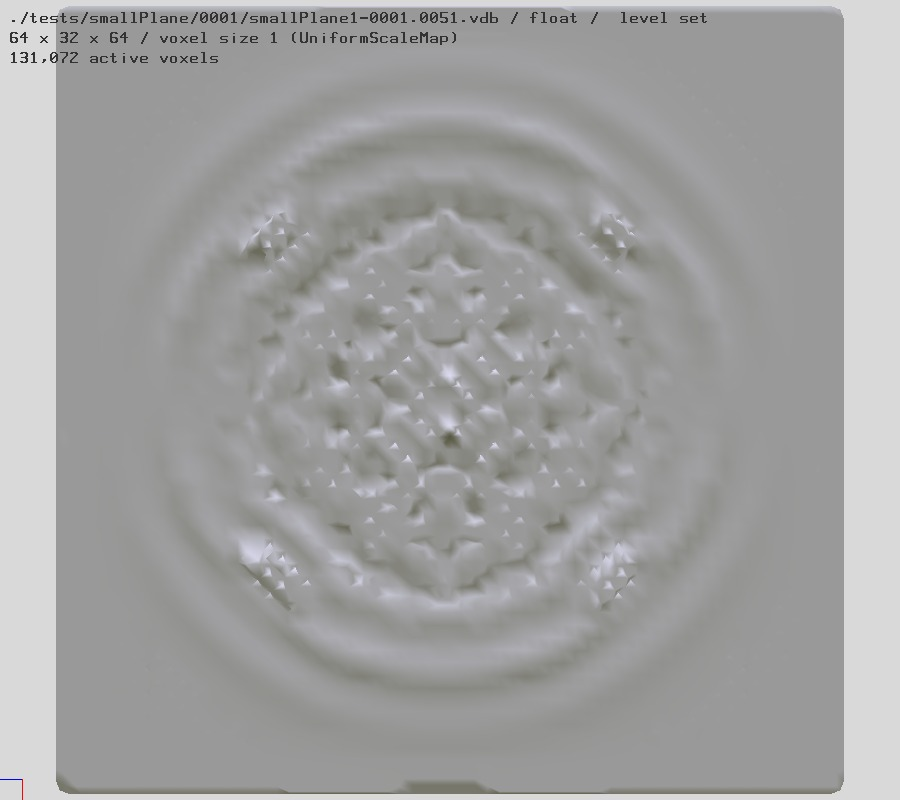
\includegraphics[width=1.5in]{../graphics/wedge1/garret2_width4_dxhi.jpg} &
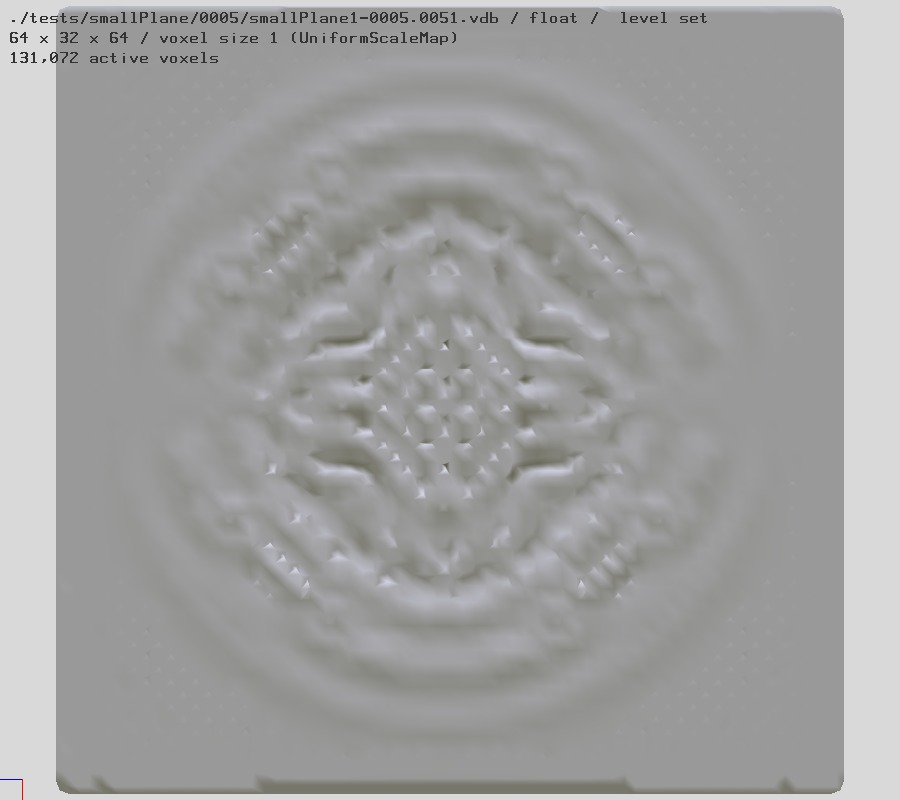
\includegraphics[width=1.5in]{../graphics/wedge1/garret2_width6_dxhi.jpg} &
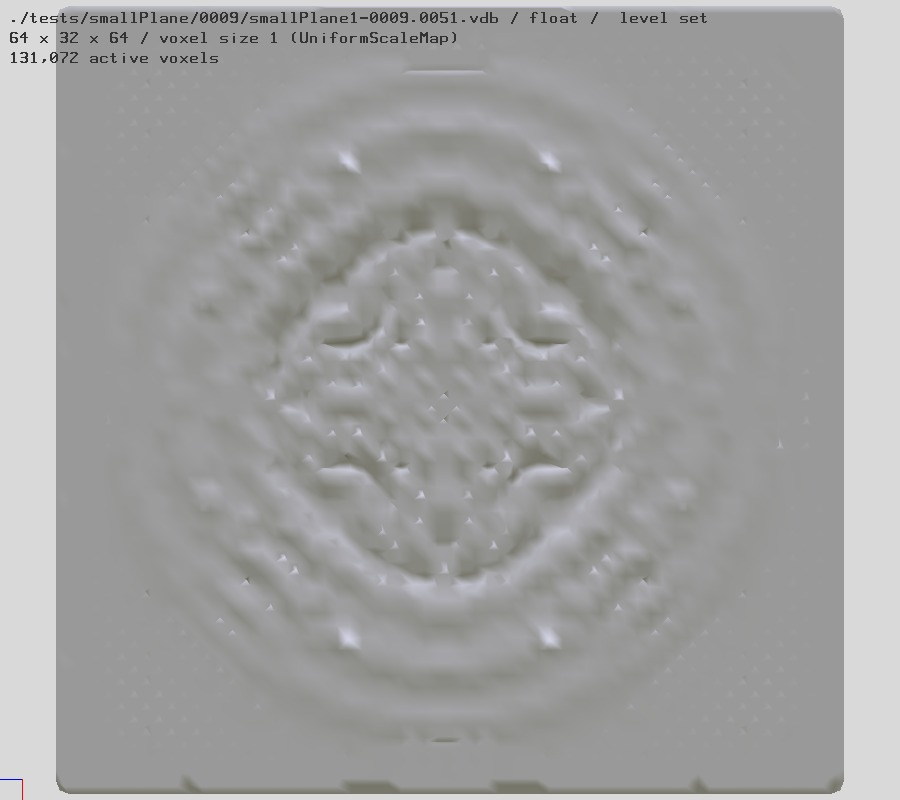
\includegraphics[width=1.5in]{../graphics/wedge1/garret2_width8_dxhi.jpg} &  Garrett2\\
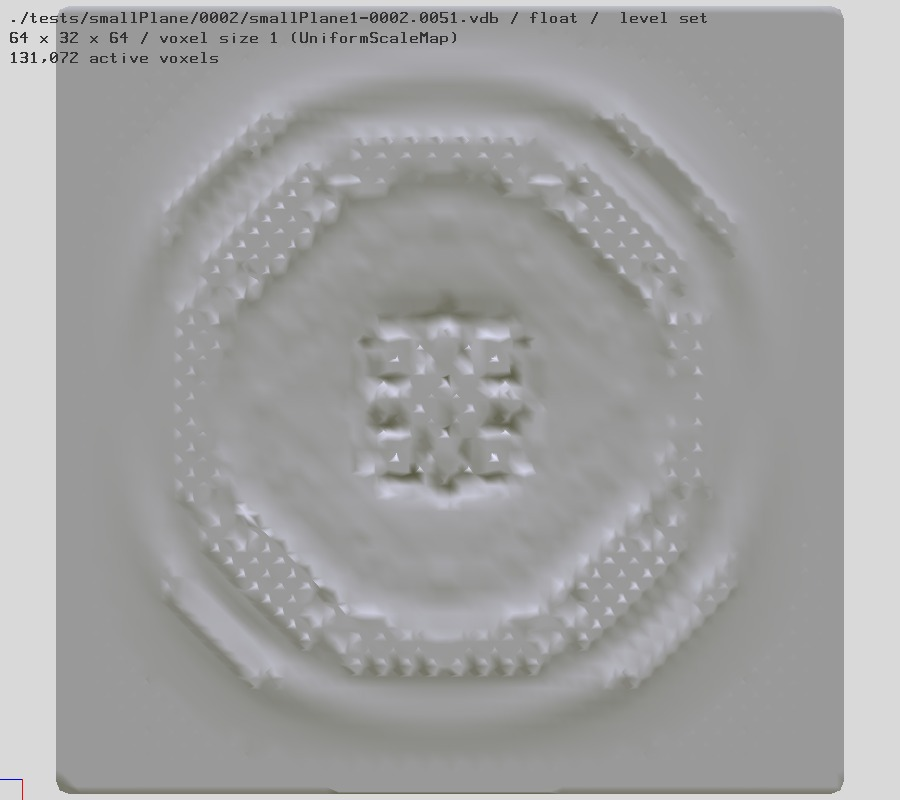
\includegraphics[width=1.5in]{../graphics/wedge1/garret4_width4_dxhi.jpg} &
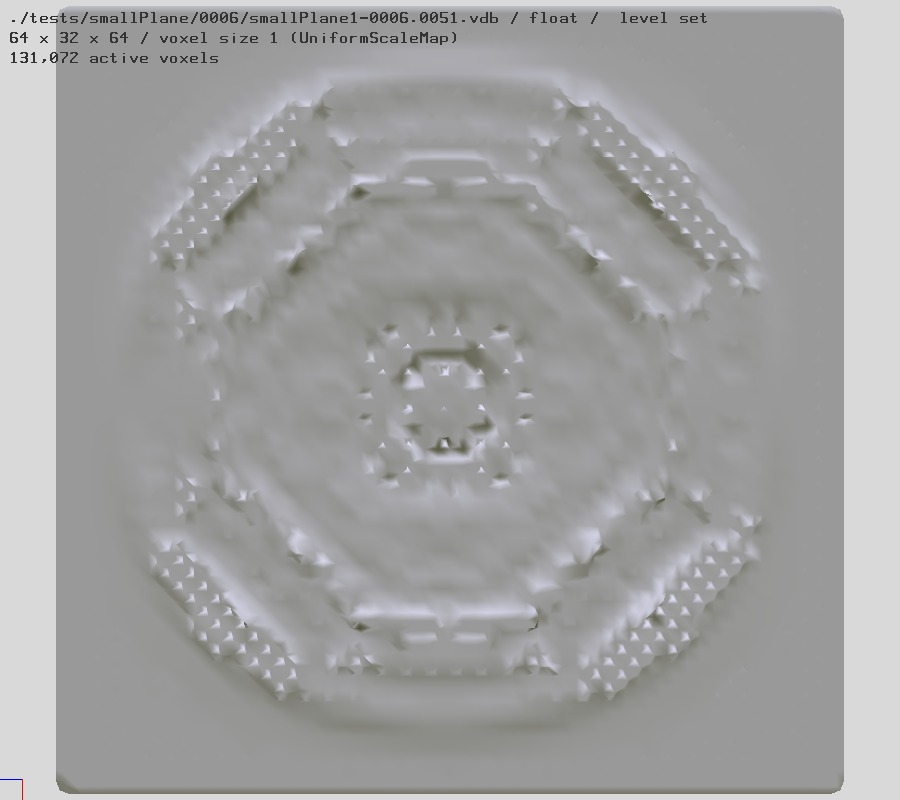
\includegraphics[width=1.5in]{../graphics/wedge1/garret4_width6_dxhi.jpg} &
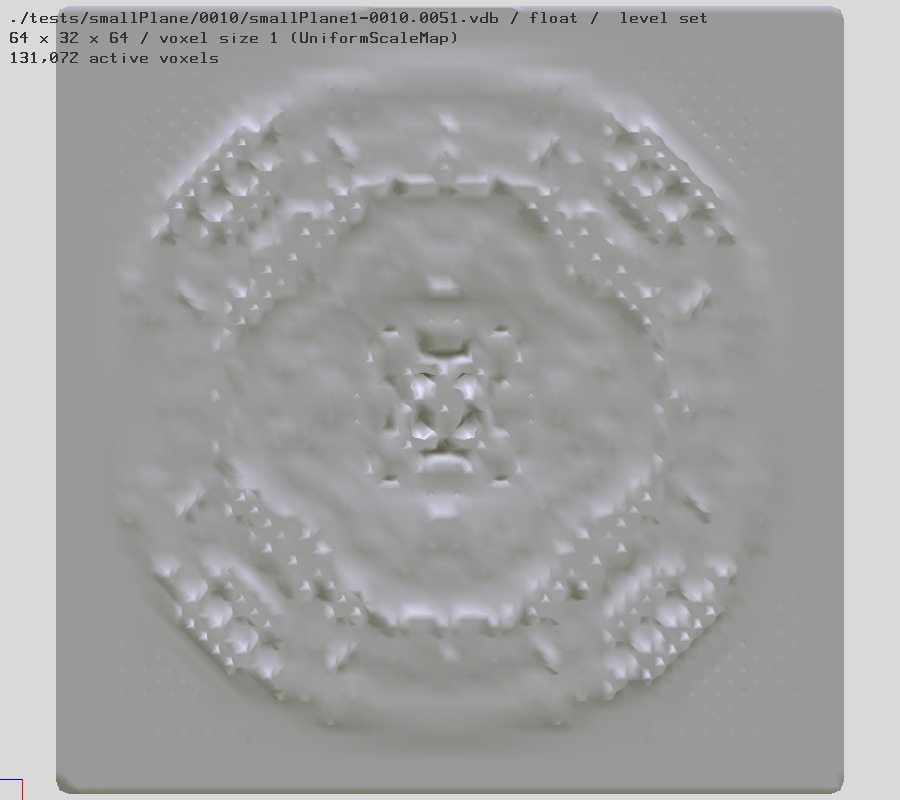
\includegraphics[width=1.5in]{../graphics/wedge1/garret4_width8_dxhi.jpg} &  Garrett4\\
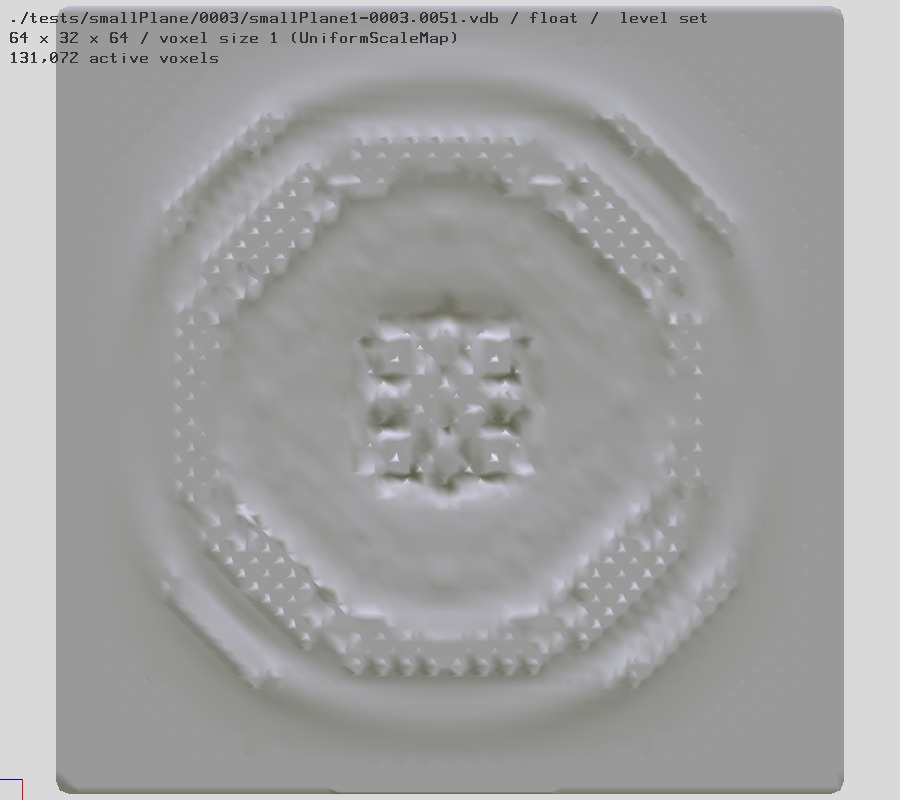
\includegraphics[width=1.5in]{../graphics/wedge1/garret6_width4_dxhi.jpg} &
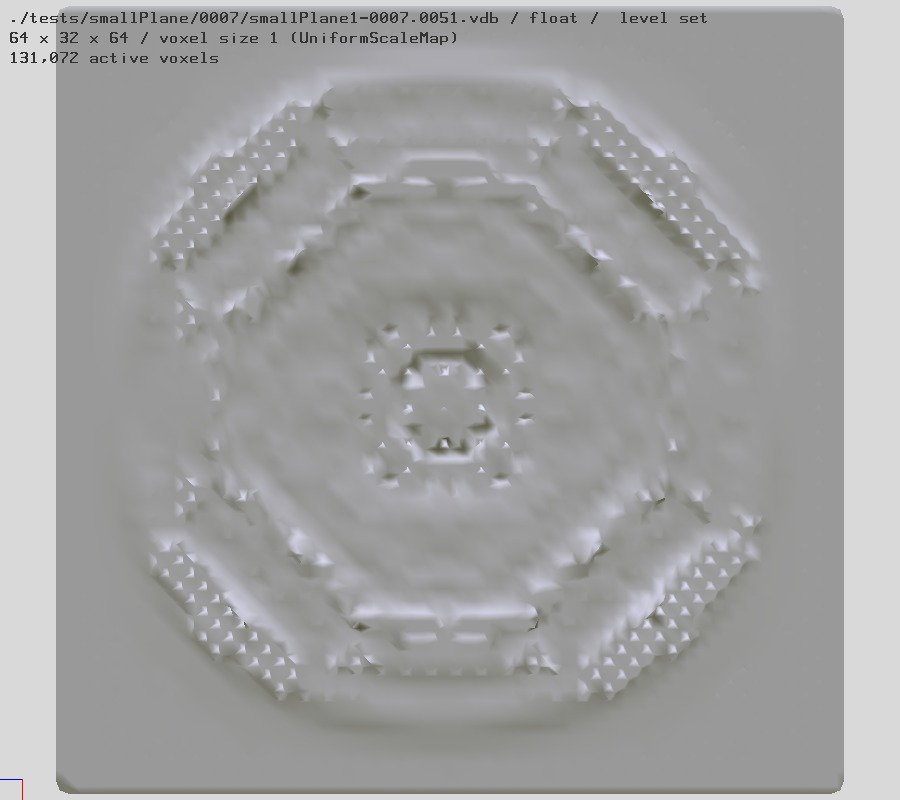
\includegraphics[width=1.5in]{../graphics/wedge1/garret6_width6_dxhi.jpg} &
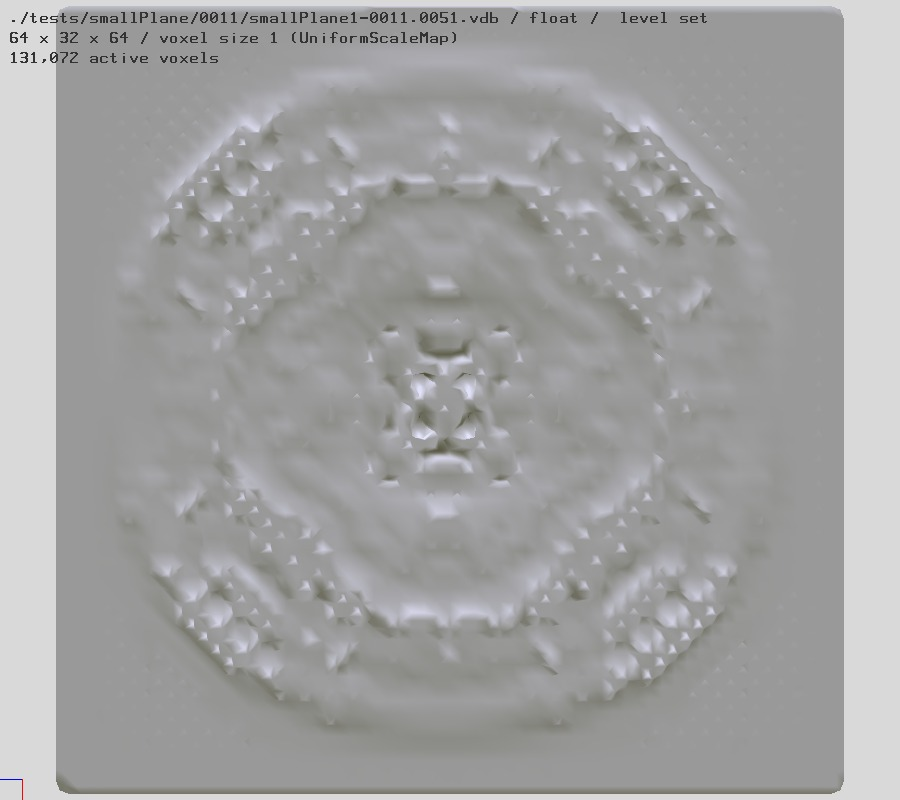
\includegraphics[width=1.5in]{../graphics/wedge1/garret6_width8_dxhi.jpg} &  Garrett6\\
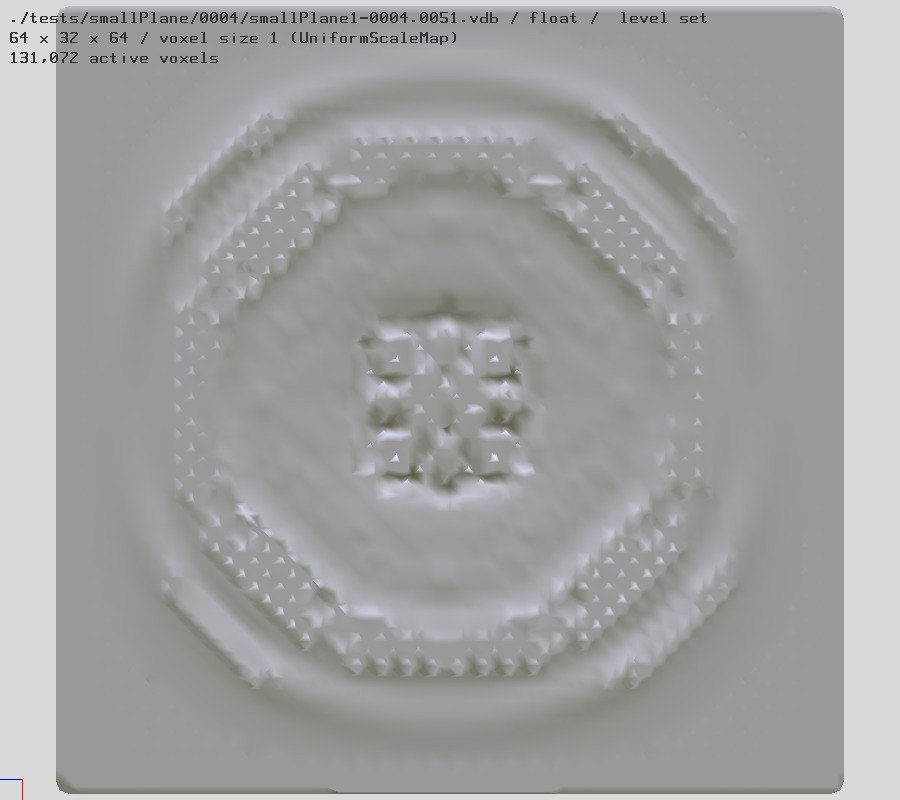
\includegraphics[width=1.5in]{../graphics/wedge1/garret8_width4_dxhi.jpg} &
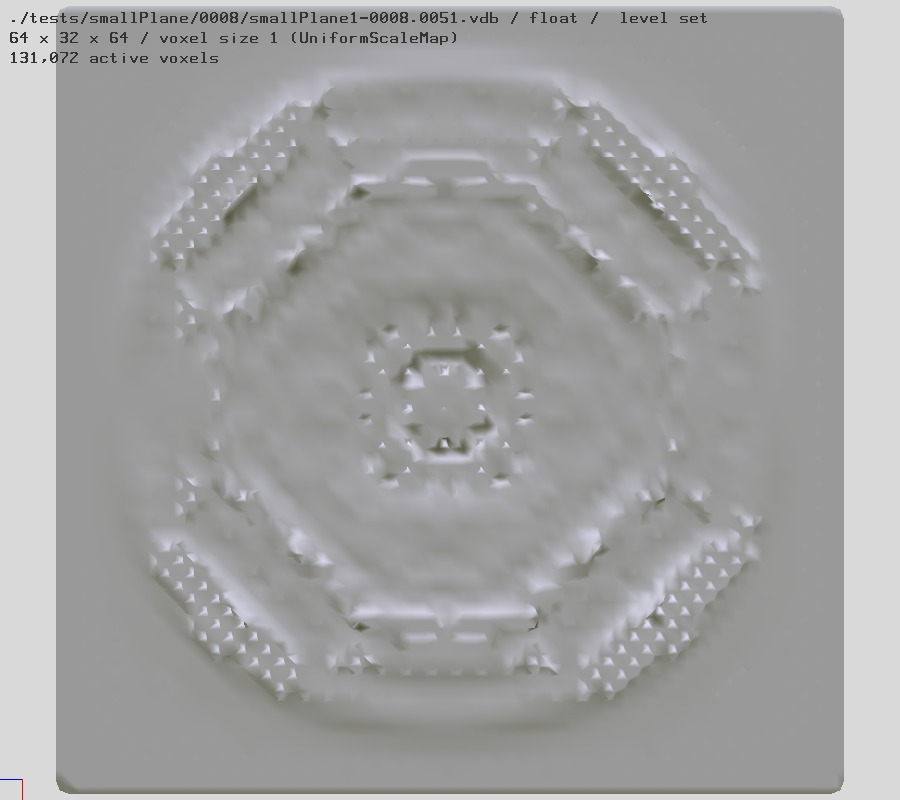
\includegraphics[width=1.5in]{../graphics/wedge1/garret8_width6_dxhi.jpg} &
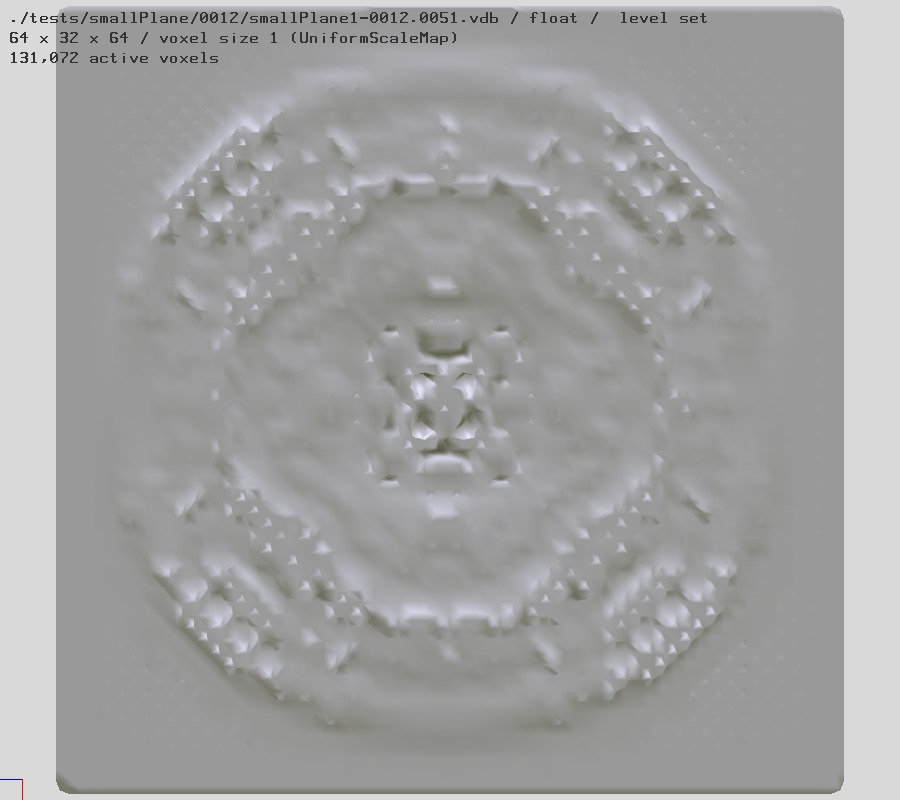
\includegraphics[width=1.5in]{../graphics/wedge1/garret8_width8_dxhi.jpg} &  Garrett8
\end{tabular}
\end{center}
\caption{ Wedge of simulation parameters for gradient order and garret solver order. These are frame 51 of the simulation. The simulation domain is $3 m \times 1.5 m \times 3m$, cell size is $0.046875 m$. Spikes less than one voxel have been eroded. Top row: Garrett2 solver. Finite difference order is (left to right) 4, 6, 8.  Second row: Garrett4 solver. Finite difference order is (left to right) 4, 6, 8.  Third row: Garrett6 solver. Finite difference order is (left to right) 4, 6, 8.  Bottom row: Garrett8 solver. Finite difference order is (left to right) 4, 6, 8.    } \label{wedge1fig}
\end{figure}


Figure \ref{spherewedgefig} shows frame 65 of the simulation on a sphere.  Erosion by even one voxel substantially suppresses the spiky features, as seen by comparing \ref{spherewedgefig}(a) with \ref{spherewedgefig}(b).  This is not to say that the spiky features are artifacts however.  They might very well be dynamically correct behavior, but the low resolution may make it difficult for the dynamics to produce a natural shape. As some evidence of that, figure \ref{spherewedgefig}(c) shows the same frame with higher spatial resolution and with one voxel erosion, but now some spiky features persist and assume shapes and motion more like splashes.  Even higher resolution is needed to clearly determine the effect.  
\begin{figure}
\begin{center}
\begin{tabular}{ccc}
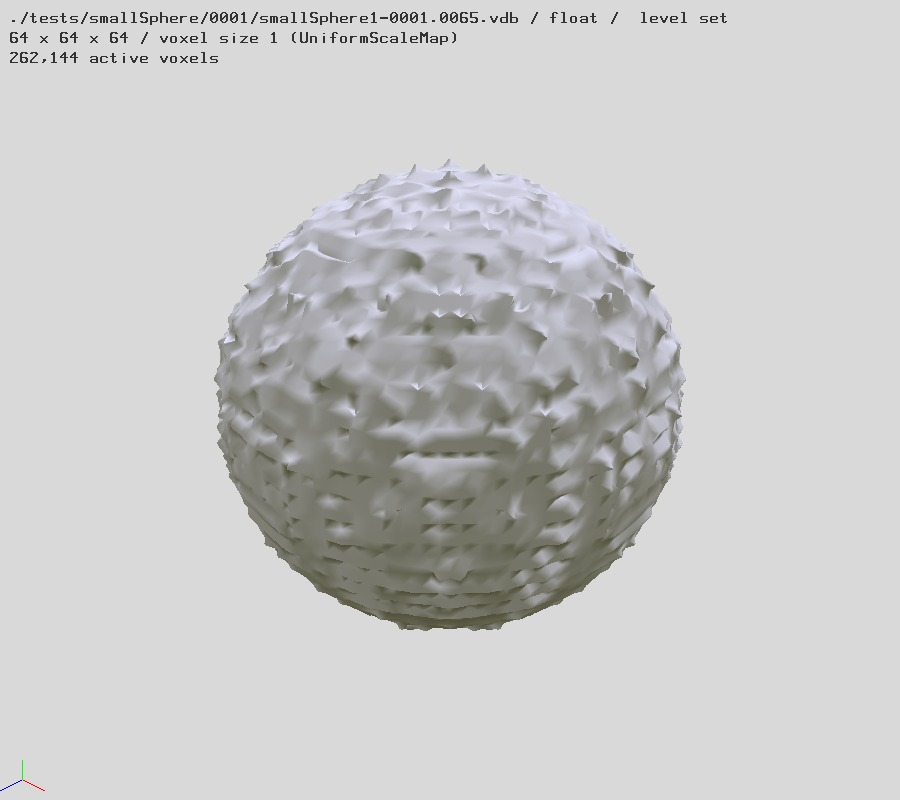
\includegraphics[width=1.5in]{../graphics/sphere_lowres_noteroded.jpg} &
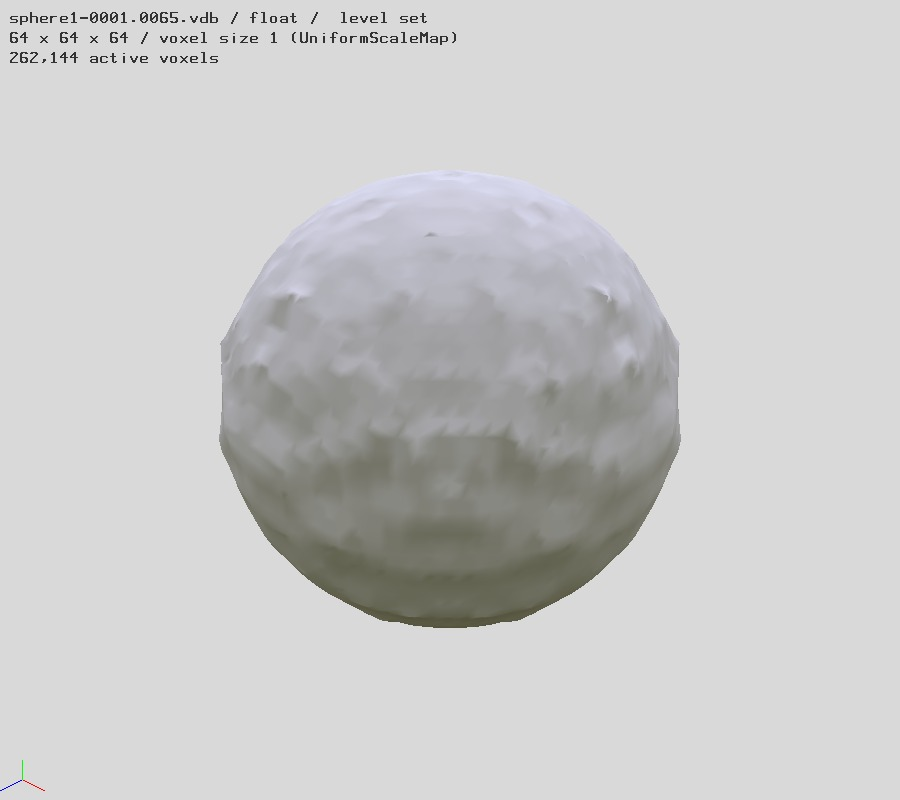
\includegraphics[width=1.5in]{../graphics/sphere_lowres_eroded.jpg} &
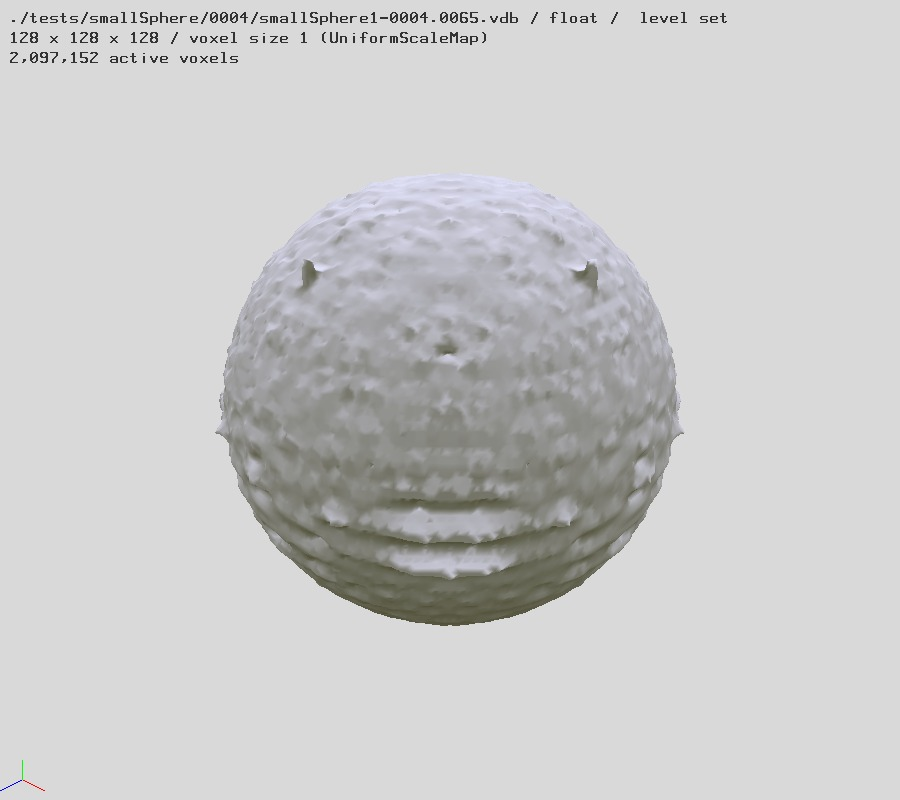
\includegraphics[width=1.5in]{../graphics/sphere_hires_eroded.jpg} \\
(a) & (b) & (c)
\end{tabular}
\end{center}
\caption{ Frame 65 of a simulation on a sphere. The simulation domain is $3 m \times 1.5 m \times 3m$. Garrett2 solver, with 4th order finite difference. 
(a) Cell size is $0.046875 m$, and no erosion.
(b) Cell size is $0.046875 m$, and there is one voxel of erosion.
(c) Cell size is $0.0234375 m$, and there is one voxel of erosion. Note the surviving spikes that may be splash-like.
  } \label{spherewedgefig}
\end{figure}

In all simulations on the sphere and plane, the solution remains finite and well-behaved without subframe stepping.  

\section{Derivation}\label{derivation}

The nbWave equations \ref{phieqn} - \ref{seqn} follow from perturbing a solution of the Navier-Stokes equations, and looking for a potential flow solution for the pertubation.  A base velocity field $\uvec_B(\xvec,t)$, base implicit field for the surface $S_B(\xvec,t)$, and base displacement vector field $\Xvec_B(\xvec,t)$ are assumed, and satisfy the following equations
\begin{eqnarray}
\frac{\partial \uvec}{\partial t}\ +\ \uvec\cdot\nabla\uvec \ +\ \nabla P &=& \fvec \\
\frac{\partial S}{\partial t}\ +\ \uvec\cdot\nabla S &=& 0 \\
\frac{\partial \Xvec}{\partial t}\ +\ \uvec\cdot\nabla\Xvec &=& 0 \\
\nabla\cdot\uvec &=& 0
\end{eqnarray}
These fields may have been created using additional dynamical or constraint equations with additional physics or effects.  The perturbation fields $\phi,\ S_E,\ \Xvec_E$ apply as $\uvec = \uvec_B + \nabla\phi$, $S = S_B + S_E$, $\Xvec = \Xvec_B + \Xvec_E$.  Applying the equations of motion and expressing them as equations for the perturbing fields, 
\begin{eqnarray}
\frac{\partial \phi}{\partial t}\ +\ \uvec_B\cdot\nabla\phi\ +\ \frac{1}{2}\left| \nabla\phi \right|^2 \ +\ P &=& f_E \\
\frac{\partial S_E}{\partial t}\ +\ (\uvec_B+\nabla\phi)\cdot\nabla S_E &=& -\nabla S_B\ \cdot\ \nabla\phi \\
\frac{\partial \Xvec_E}{\partial t}\ +\ (\uvec_B+\nabla\phi)\cdot\nabla\Xvec_E &=& -(\nabla\Xvec_B)^{T}\cdot\nabla\phi \\
\nabla^2\phi &=& 0
\end{eqnarray}
From here, there are several reduction items:
\begin{enumerate}
\item All of the fields are advected by the base velocity. This advection can be applied as a separate option before or after the other dynamics in these equations. These equations are reduced accordingly by removed the terms involving $\uvec_B\cdot\nabla$.  
\item The pressure is involved in enforcing incompressibility.  Incompressibility is enforced by using an incompressible gradient.  This means the pressure field can be removed from the equations.
\item The based simulation displacement is just the identity $\Xvec_B = \xvec$, and the gradient $\nabla\Xvec_B$ is the identity matrix. 
\item The Laplace equation for incompressibility is enforced by replacing all of the $\nabla\phi$ terms with incompressible gradients $\inabla\phi$.
\item The equations for eWave are the linearized dynamical equations. Nonlinear dynamics could be considered at some point, but presently only linear dynamics is involved.  
\end{enumerate}
With these reductions, the equations become
\begin{eqnarray}
\frac{\partial \phi}{\partial t} &=& f_E \\
\frac{\partial S_E}{\partial t}  &=& -\nabla S_B\ \cdot\ \inabla\phi \\
\frac{\partial \Xvec_E}{\partial t} &=& -\inabla\phi \\
\end{eqnarray}
The forcing term $f_E$ for gravity is driven by displacement of the surface from the base solution.  This is tracked by the displacement field $\Xvec_E$.  For gravity, the forcing is
\begin{equation}
f_E \ =\ -\gvec\cdot\Xvec_E
\end{equation}


\section{Additional Effort}

There are several addition efforts that are worthwhile pursuing to characterize this simulation approach, and possibly improve it:
\begin{enumerate}
\item Evaluate the impact of subframe stepping.  Subframe stepping is not likely to improve stability, but transient and spiky features may acquire more natural shapes.
\item Evaluate the transition to higher resolution and larger simulation domains.  
\item Restore nonlinear terms in the equations and evaluate the change in stability, motion and structure.
\end{enumerate}


\end{document}
